%
% File emnlp2020.tex
%
%% Based on the style files for ACL 2020, which were
%% Based on the style files for ACL 2018, NAACL 2018/19, which were
%% Based on the style files for ACL-2015, with some improvements
%%  taken from the NAACL-2016 style
%% Based on the style files for ACL-2014, which were, in turn,
%% based on ACL-2013, ACL-2012, ACL-2011, ACL-2010, ACL-IJCNLP-2009,
%% EACL-2009, IJCNLP-2008...
%% Based on the style files for EACL 2006 by 
%%e.agirre@ehu.es or Sergi.Balari@uab.es
%% and that of ACL 08 by Joakim Nivre and Noah Smith

\documentclass[11pt,a4paper]{article}
\usepackage[hyperref]{emnlp2020}
\usepackage{times}
\usepackage{latexsym}
\renewcommand{\UrlFont}{\ttfamily\small}

\usepackage{graphicx}
\usepackage{xcolor}
\usepackage{longtable}
\usepackage{tikz}
\usetikzlibrary{calc}
\usepackage[draft]{todo}
\usepackage{xspace}
\usepackage{amsmath,amsfonts,amssymb}
\usepackage{mathrsfs}
\newcommand{\R}{\ensuremath{\mathbb{R}}}

% This is not strictly necessary, and may be commented out,
% but it will improve the layout of the manuscript,
% and will typically save some space.Boldface denotes significant gains with respect to \system{Mix-Nat} (or \system{Mix-Nat-RNN}, for WDCMT), underline denotes significant losses.
\usepackage{microtype}

%\aclfinalcopy % Uncomment this line for the final submission
%\def\aclpaperid{***} %  Enter the acl Paper ID here

%\setlength\titlebox{5cm}
% You can expand the titlebox if you need extra space
% to show all the authors. Please do not make the titlebox
% smaller than 5cm (the original size); we will check this
% in the camera-ready version and ask you to change it back.

\newcommand{\fyTodo}[1]{\Todo[FY:]{\textcolor{orange}{#1}}}
\newcommand{\fyTodostar}[1]{\Todo*[FY:]{\textcolor{orange}{#1}}}
\newcommand{\fyDone}[1]{\done[FY]\Todo[FY:]{\textcolor{orange}{#1}}}
\newcommand{\fyFuture}[1]{\done[FY]\Todo[FY:]{\textcolor{red}{#1}}}
\newcommand{\fyDonestar}[1]{\done[FY]\Todo[FY:]{\textcolor{orange}{#1}}}
\newcommand{\jcTodo}[1]{\Todo[JC:]{\textcolor{red}{#1}}}
\newcommand{\jcDone}[1]{\done[JC]\Todo[JC:]{\textcolor{red}{#1}}}

\newcommand{\mpTodo}[1]{\Todo[MP:]{\textcolor{green}{#1}}}
\newcommand{\mpDone}[1]{\done[MP]\Todo[MP:]{\textcolor{green}{#1}}}
\usepackage{mathtools,xparse}
\DeclarePairedDelimiter{\abs}{\lvert}{\rvert}
\DeclarePairedDelimiter{\norm}{\lVert}{\rVert}
\NewDocumentCommand{\normL}{ s O{} m }{%
  \IfBooleanTF{#1}{\norm*{#3}}{\norm[#2]{#3}}_{L_2}%
}
\newcommand{\src}{\ensuremath{\mathbf{f}}} % source sentence
\newcommand{\trg}{\ensuremath{\mathbf{e}}} % target sentence
\newcommand{\domain}[1]{\texttt{\textsc{#1}}}
\newcommand{\system}[1]{\texttt{\textbf{#1}}}
\newcommand{\vlambda}{\ensuremath{\boldsymbol\lambda}\xspace} % parameters vector for a distribution
\newcommand{\indic}[1]{\ensuremath{\mathbb{I}(#1)}}
% \newcommand{\SB}[1]{\textcolor{green}{#1}}
% \newcommand{\SW}[1]{\textcolor{red}{#1}}
\newcommand{\SB}[1]{\textbf{#1}}
\newcommand{\SW}[1]{\underline{#1}}
\renewcommand\textfraction{.1}
\renewcommand\floatpagefraction{.95}

\newcommand\BibTeX{B\textsc{ib}\TeX}

\title{Ablation study on the residual adapter in Neural Machine Translation}

\author{First Author \\
  Affiliation / Address line 1 \\
  Affiliation / Address line 2 \\
  Affiliation / Address line 3 \\
  \texttt{email@domain} \\\And
  Second Author \\
  Affiliation / Address line 1 \\
  Affiliation / Address line 2 \\
  Affiliation / Address line 3 \\
  \texttt{email@domain} \\}

\date{}

\begin{document}
\maketitle
\begin{abstract}
Among the approaches for adapting a pretrained NMT model to a specific domain, finetuning is the dominant method. Finetuning proposes 2 approaches: simply continuing training all the parameters \cite{Luong15stanford}; training addition adapters while freezing the pretrained model\cite{Bapna19simple, Vilar18learning}. The second approach has several advantages including preserving the pretrained model and the legerity of the adapters. However, the behavior of these adapters has not been further studied. The objective of this paper is to give an ablation study on the use of residual adapter in the domain adaptation problem.
\mpTodo{correcting abstract}

**** 

\fyTodo{Citation-free abstract}
Domain adaptation is an old and vexing problem for machine translation systems. The most common approach and successful to supervised adaptation is to fine-tune a baseline system with in-domain parallel data. Standard fine-tuning however modifies all the network parameters, which makes this approach computationally costly and prone to overfitting. A recent, lightweigth approach, instead augments a baseline model with supplementary (small) adapter layers, keeping the rest of the mode unchanged. This has the additional merit to leave the baseline model intact, and adaptable to multiple domains. In this paper, we conduct a thorough analysis of the adapter model in the context of a multidomain machine translation task. We contrast multiple implementations of this idea on two language pairs. Our main conclusions is ..\fyTodo{abstract to be continued}

\end{abstract}
\section{Introduction } \label{sec:intro}
\mpTodo{write introduction} \fyTodo{Citations in chronological order}\fyTodo{Split long sentences}
Owing to multiple architectural improvements, Neural Machine Translation(NMT) \cite{Kalchbrenner13recurrent,Sutskever14sequence,Bahdanau15learning,Vaswani17attention} nowadays delivers useful outputs for many language pairs. However, as many deep learning model, NMT models need to be trained with sufficiently large amounts of data to reach their best performance. Therefore, the quality of translation of NMT model is still limited in low-resource language and low-resourced domain conditions \cite{duh13adaptation, zoph16transfer,koehn17six}. While many approaches have been proposed to improve the quality of NMT models in low-resource domains (see the recent survey of \citet{Chu18asurvey}), full fine-tuning of a generic baseline model remains the dominant supervised approach when adapting NMT models to specific domains \cite{Luong15stanford,neubig18rapid}.

Under this view, building adapted systems is a two-step process: (a) one first trains NMT with the largest possible parallel corpora, possibility aggregating texts from multiple, heterogeneous sources; (b) assuming that in-domain parallel documents are available for the domain of interest, one then adapts the pretrained model by resuming training with the sole in-domain corpus. It is a conjecture that pretrained model constitute a better initialization a the random initialization, especially when the adaptation data is scarce. Indeed, studies in transfer learning for NMT such as \cite{artetxe20cross,aji20neural} have confirmed this claim by extensive experiments. Full fine-tuning, that is adapting all the parameters of a baseline model usally significantly improves the quality of the NMT for the chosen domain. However, it also implies large losses in translation quality for other domains, a phenomenon referred to as ``catastrophic forgetting'' in the neural network literature \cite{McCloskey89catastrophic}. Therefore, a fully fine-tuned model is only useful to one target domain. As the number of domains to handle grows, training and maintaining such models can consume a lot of resource.\fyTodo{Fix this sentence}

\cite{Vilar18learning,bapna19simple} have recently proposed a simple and lightweight method to preserve the value of pretrained models by plugging small adapters to hidden layers. These adapters are trained only with the in-domain data, keeping the pretrained model frozen. Because these additional adapters are very small compared to the size of the baseline model, their use significantly reduces the cost of training and maintaining fine-tuned models, while still delivering a performance that is on par with full fine-tuning.

In this paper, we would like to extend this architecture to improve NMT in several specific situations that still challenge automatic translation, such as translating noisy inputs or translating topical texts\fyTodo{??}. Residual adapters allow us to adapt NMT model to any specific domain in a computationally economical way. Could we adapt NMT model to noisy text and topical text at once? While residual adapters are good at adapting to one specific domain, their performance still dramatically decrease for the other domains seen in training, as we show in our experiments. Therefore, we have to decide whether to use residual adapters manually, i.e, we have to know to which domain the text belongs a priori. Therefore, we would like to fuse a domain classifier to the architecture in order to weight the contribution of the adapters with respect to the topic-relatedness of the text.\fyTodo{Say differently: various implementations}

Our contribution is an thorough experimental study on the use of residual adapters in multidomain adapation. We notably try to answer the following three questions:
\begin{itemize}
\item How the number and position of adapters affect the performance.
\item How to train the residual adapters.
\item How to render the combination of NMT model and residual adapters more robust to out-of-domain examples.
\end{itemize}
\fyTodo{One bit of a conclusion here}

\section{Residual adapters \label{sec:res}}

\subsection{Architecture \label{ssec:architecture}}
\fyTodo{More contexts and notations from the transformer}

Residual adapters modify context vectors in each layer by applying several transformations as follows:\fyTodo{Use align env}
\begin{align*}
  h^{i}_1 &= \mathbf{W}_{d_{model}}^{d_{bottleneck}}h^{i} + b_{1} \\
  h^{i}_2 &= \mathbf{RELU}(h_1) \\
  h^{i}_3 &= \mathbf{W}_{d_{bottleneck}}^{d_{model}}h_2 + b_{2} \\
  \bar{h}^{i} &= h^i_3 + h^i
\end{align*}
For the sake of brevity, we denote $h^i_3 = \operatorname{ADAP}^{(i)}(h^i)$.\fyDone{or is it $h_i$ ?}

The "adapted" context vector $\bar{h}^i$ goes to\fyTodo{Is the output of ?} the $(i+1)^{\text{th}}$ attention\fyDone{Self attention ?} layer. In our architecture, there are 12 residual adapters, one for each of the six attention layers of the encoder and similarly for the decoder\footnote{In the decoder, the stack of self-attention layers and cross encoder-decoder attention only counts as one attention layer and serves only one residual adapter}.

\subsection{Ablation study on position and number of residual adapters \label{ssec:ablatation}}
In this section, we would like to analyze the impact of position and number of residual adapters involved in the adapted model. In fact, the importance of hidden layers varies with respect to their position in the model. It is conjectured that the higher layer represents more global pattern such as syntax while the lower layer represents more local pattern such as semantic\fyTodo{Missing reference here}. The domain shift in local patterns and global patterns has not yet studied. In this paper, we do not intend to study this aspect of domain adaptation problem. We would like to give an extensive comparison between domain adaptation in different levels in NMT model.\fyTodo{Fix style here} Because the set of possible configurations is large, we only perform experiments on layers at position: 2, 4, 6 which covers a wide range in the hierarchy of attention layers. 

Second, we would like to observe how much the number of residual adapters affects the performance of the adapted model. By the limit of computation resource, we limit our study to the case of 3 adapters at positions: 2,4,6. By doing this, we could cover 3 situations: 1 adapter (mentioned in the previous paragraph), 3 adapters and 6 adapters (in the normal setting) in the encoder or the decoder.\fyTodo{We have 12 layers, have we not ?}

Finally, we would like to assess the performance of a variant of residual adapters in which the adapters go directly to the end of the stack of attention layers. We graphically demonstrate this version in the figure \ref{fig:hrl-architecture}. The benefit of this variant is that we can manipulate all values of the adapters at once. An disadvantage of this variant is a lower complexity than original version because the change of context vector only occurs in the end of the stack of layers.

\subsection{Regularization of residual adapters \label{ssec:reg}}
Fine-tuning on small corpora can still lead to overfitted model even when the fine-tuning is applied to a few residual adapters. To avoid this situation, we have several options including: reduce the size of the adapter module, apply weight decay to the adapter during adaptation, or apply layer regularization to the adapter modules. The first option is not flexible \fyTodo{compatible ???} if we consider the probable growth of in-domain data. The second and third choices are preferable to regularize a large adapter which will scale if the in-domain corpora extends.\fyTodo{Style}

Weight decay applies a penalization on weights of the adapters.
\begin{equation}
  \begin{split}
    \bar{L} & = \mathop{\sum}_{x,y} (log(P(y|x)) \\
    & + \lambda * \sum_{i \in \{1,..,6\} \otimes \{enc, dec\}} \normL{\theta_{\operatorname{ADAP}^{(i)}}})
  \end{split}
\end{equation}

Layer regularization applies a penalization on the output of the adapters.
\begin{equation}
  \begin{split}
    \bar{L} & = \mathop{\sum}_{x,y} (log(P(y|x)) \\
    & + \lambda * \sum_{i \in \{1,..,6\} \otimes \{enc, dec\}} \normL{\operatorname{ADAP}^{(i)}(h_i(x,y))})
  \end{split}
\end{equation}

\subsection{Multi-task training\label{ssec:multitask}}
In the experiments of \cite{Caruana97multitask}, the authors proposed an architecture suitable for multi-task learning. The corresponding network comprises a ground layer, which is shared between tasks and is followed by task-related layers in the next level. The network is then trained from scratch by fueling task-related examples in a batch and updating all parameters (shared and task-specific) at the same time. The multi-domain context is similar to multi-task context if we consider a domain as a task\cite{Dredze08}. Therefore, we can also use multi-task training to optimize the parameters of NMT model and the parameters of the residual adapters at once from beginning. To assess the efficacy of multi-task training in multi-domain context, we would like to compare the finetuning approach with multi-task training approach. \fyTodo{Change the training regime}

\subsection{Word-Level Adaptive Domain Adaptation \label{ssec:wada}}
\mpTodo{Formalizing problem, network design, training algorithm}
Residual adapters allow us to adapt NMT models to a new domain without altering the pretrained parameters. However, we still have to decide in which domain a sentence is translated to chose a suitable adapter.\fyTodo{Lack of context - domain errors} Therefore, we face to another problem which is the error of domain prediction. Choosing wrong adapter to translate a sentence can be dramatically bad because a specialized model usually has bad performance for out-of-domain instances \cite{McCloskey89catastrophic}. However, we still have another option that is to use the pretrained generic model without adaptation. Therefore, we could aim to achieve a performance at least as good as the generic model. We would like to present an adaptive version of residual adapter below.

We consider a generic encoder-decoder architecture for a multi-domain sequence to sequence learning. Let $h \in \R^d$ the output of the encoder, \cite{bapna19simple} proposes to use an adapted representation for domain $k$ defined as $h' = h + a_k(h)$. This means that all words in all sentences in domain $k$ will use the adapter module represented by $a_k$. In a multilayer version with highway connections (see Figure~\ref{fig:hrl-architecture}), $a_k(h) = \sum_{l} a_{kl}(h^l)$ where $h^l$ is the distributed representation of the sequence at the $l^{th}$ layer.
\begin{figure}[htbp]
  \centering
  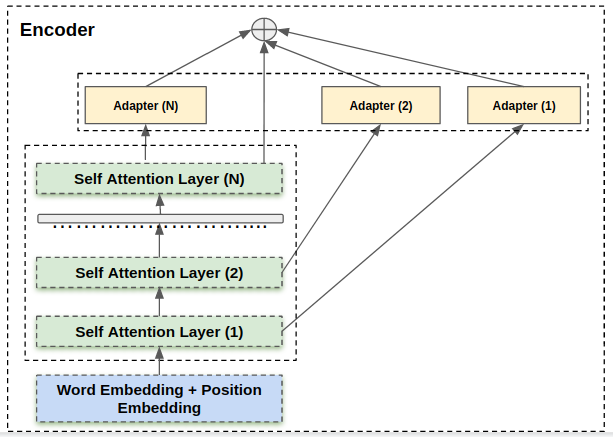
\includegraphics[scale=0.3]{fig/highway_residual}
  \caption{Highway multi-domain network with residual layers}
\label{fig:hrl-architecture}
\end{figure}

A "gated" version uses $h' = h + a_k(h) \odot{} z_k(h)$\footnote{Or $a_k(h) = \sum_{l} a_{kl}(h)$, where the summation runs over layers, see Figure~\ref{fig:hrl-architecture}} where $z_k$ is a function of $h$ taking values in $[0,1]$. More precisely, $h$ and $h'$ are sequences of context vectors and the combination is performed element-wise, yielding:
\begin{equation}
   \forall t \in [1 \dots{} T], h'(w_t) = h(w_t) + a_k(h(w_t)) \odot{} z_k(h(w_t)). \label{eq:gated-residual}
\end{equation}

In Word Level Adaptive Domain Adaptation (WADA), $z_k(h(w))$ is designed to reflect the "topicality" of  word $w$ is in domain $k$: the more likely $w$ is in domain $k$, the larger $z_k(h(w))$ should be. Word-level adaptive domain adaptation aims to reduce the variation caused by $a_k$ to the adapted context vector $h'$ (compared to $h$) for words that are not typical of domain $k$. By reusing the learned generic representation for non-topical words, we can bound the risk of poor predictions in case of out-of-domain words by the risk of the learned generic model.

\subsubsection{The training process \label{sssec:train}}
The training process comprises three main steps:
\begin{itemize}
	\item Pretraining a generic model with a mixed corpora comprising data from multiple domains.
	\item Training a domain classifier on top of the encoder and decoder; during this step, the parameters of the generic model are frozen. This model computes the posterior domain probability $p(k|h(w_t))$ for each word $w_t$ based on the representation computed by the last layer.
	\item Training the parameters of adapters with in-domain data separately for each domain while freezing the parameters of the generic model and of the domain classifiers.
\end{itemize}
During inference, $z_k$ is used to regulate the strength of the adapter module as suggested in equation~\ref{eq:gated-residual}.

\section{Experimental settings \label{sec:exp}}
\subsection{Data and metrics \label{ssec:corpora}}
We experiment with translation from English into French and use texts initially originating from 6~domains, corresponding to the following data sources: the UFAL Medical corpus V1.0 (\domain{med})\footnote{\url{https://ufal.mff.cuni.cz/ufal_medical_corpus}}, the European Central Bank corpus (\domain{bank}) \cite{Tiedemann12parallel}; The JRC-Acquis Communautaire corpus (\domain{law}) \cite{Steinberger06acquis}, documentations for KDE, Ubuntu, GNOME and PHP from Opus collection \cite{Tiedemann09news}, collectively merged in a \domain{it}-domain, Ted Talks (\domain{talk}) \cite{Cettolo12wit}, and the Koran (\domain{rel}). Complementary experiments also use v12 of the News Commentary corpus (\domain{news}). Corpus statistics are in Table~\ref{tab:Corpora-en-fr}.  Most corpora are available from the Opus web site.\footnote{\url{http://opus.nlpl.eu}} These corpora were deduplicated and tokenized with in-house tools. To reduce the number of types and build open-vocabulary systems, we use Byte-Pair Encoding \cite{Sennrich16BPE} with 30,000 merge operations on a corpus containing all sentences in both languages.%

\begin{table*}[htbp]
  \centering
  \begin{tabular}{ |lllllll|} %*{4}{|r|}}
    \hline
    %\multicolumn{4}{|l|}{Vocab size - En: 30,165, Fr: 30,398}\\
    \domain{med} & \domain{law} & \domain{bank} & \domain{it} & \domain{talk} & \domain{rel} & \domain{news} \\
    \hline
    2609 (0.68) & 190 (0.05)  & 501 (0.13) & 270 (0.07) & 160 (0.04) & 130 (0.03) & 260 (0) \\
    \hline
  \end{tabular}
\caption{Corpora statistics: number of parallel lines ($\times 10^3$) and proportion in the basic domain mixture (which does not include the \domain{news} domain). \domain{med} is the largest domain, containing almost 70\% of the sentences, while \domain{rel} is the smallest, with only 3\% of the data.}
\label{tab:Corpora-en-fr}
\end{table*}

We also report a part of experiments in language pair English into German. We use available corpora in the News task of WMT20\footnote{\url{http://www.statmt.org/wmt20/news.html}} including: European Central Bank corpus (\domain{bank}),  European Economic and Social Committee corpus (\domain{eco}), European Medicines Agency corpus (\domain{med})\footnote{\url{https://tilde-model.s3-eu-west-1.amazonaws.com/Tilde_MODEL_Corpus.html}}, Press Release Database of European Commission corpus, News Commentary v15 corpus, Common Crawl corpus (\domain{news}), Europarl v10 (\domain{gouv}) Tilde MODEL - czechtourism (\domain{tourism})\footnote{\url{https://tilde-model.s3-eu-west-1.amazonaws.com/Tilde_MODEL_Corpus.html}}, Paracrawl and Wikipedia Matrix (\domain{others}) \footnote{\url{https://tilde-model.s3-eu-west-1.amazonaws.com/Tilde_MODEL_Corpus.html}}. We also build a joint BPE vocabulary of size 33K for both languages. The statistics for the En-De corpora are in Table~\ref{tab:Corpora-en-de}.

\begin{table*}[htbp]
  \centering
  \begin{tabular}{ |lllllll|} %*{4}{|r|}}
    \hline
    %\multicolumn{4}{|l|}{Vocab size - En: 30,165, Fr: 30,398}\\
    \domain{bank} & \domain{eco} & \domain{med} & \domain{gouv} & \domain{news} & \domain{tourism} & \domain{other} \\
    \hline
    4(0.00022) & 2857(0.15) & 347(0.018) & 1828(0.095) & 3696(0.19) & 7(0.00039) & 10472771(0.54) \\
    \hline
  \end{tabular}
\caption{Corpora statistics: number of parallel lines ($\times 10^3$) and proportion in the basic domain mixture. \domain{news} is the largest domain, containing almost 19\% of the sentences, while \domain{bank} is the smallest, with only 0.02\% of the data.}
\label{tab:Corpora-en-de}
\end{table*}

We randomly select in each corpus a development and a test set of 1,000 lines and keep the rest for training. Development sets are used to choose the best model according to the average BLEU score \cite{Papineni02bleu}.\footnote{We use truecasing and the \texttt{multibleu} script.}\fyDone{A word about meta-parameter settings} Significance testing is performed using bootstrap resampling \cite{Koehn04statistical}, implemented in compare-mt\footnote{\url{https://github.com/neulab/compare-mt}} \cite{Neubig19compare-mt}. We report significant differences at the level of $p=0.05$.\fyDone{Fix correct p value}

\subsection{Baseline architecture \label{ssec:baseline}}
\fyTodo{Write this - settings and parameters for Mix-Nat and Full-FT}.
Our baselines are standard for multi-domain systems.\footnote{We however omit domain-specific systems trained only with the corresponding subset of the data, which are always inferior to the mix-domain strategy \cite{Britz17mixing}.} Using Transformers \cite{Vaswani17attention} implemented in OpenNMT-tf\footnote{\url{https://github.com/OpenNMT/OpenNMT-tf}} \cite{Klein17opennmt}, we build the following systems:
\begin{itemize}
\item a generic model trained on a concatenation of all corpora, denoted \system{Mixed}\fyTodo{Or mixed nat ?}
\item fine-tuned models \cite{Luong15stanford,Freitag16fast}, based on the \system{Mixed} system, further trained on each domain with early stopping when the dev BLEU stops increasing significantly in 3 consecutive epochs. We again contrast two versions: full fine-tuning (\system{FT-Full}), which update all the parameters of the initial generic model \system{Mixed}; and the variant of \cite{Bapna19simple} (\system{FT-Block}).
\end{itemize}

For all models, we set the embeddings size and the hidden layers size to~512. Transformers use multi-head attention with 8 heads in each of the 6 layers; the inner feedforward layer contains 2048 cells. The multi-domain residual system (see description below) additionally uses an adaptation block in each transformer layer, composed of 2-layer perceptron, with an inner RELU activation function operating on normalized entries of dimension 1024. 
% The gated variant is made of a dense layer, followed by a layer normalization and a sigmoid activation.
% The domain control systems are exactly as their baseline counterparts (RNN and Transformer), with an additional 2 cells encoding the domain on the input layer.
Training use a batch size of~12288 tokens; optimization uses Adam with parameters $\beta_1=0.9$, $\beta_2= 0.98$ and Noam decay ($warmup\_steps=4000$), and a dropout rate of $0.1$ for all layers.\fyDone{Describe the block adaptation layer - voir slides}

\subsection{Varying the positions and number of residual adapters}

Tables \ref{tab:Corpora-en-fr} and \ref{tab:performance-en-de} display the performace of NMT model in 6 domains: \domain{med},\domain{law},\domain{bank},\domain{talk},\domain{it} and \domain{rel} for the language pair En-Fr; \domain{gouv}, \domain{eco}, \domain{tourism}, \domain{bank}, \domain{med} and \domain{news} for En-De. In most cases, the performance increases with respect to the number of residual adapters used in architecture. The setting \system{FT-block} using residual adapters at all levels outperforms setting \system{FT-Block$_{(2,4,6)}$} using residual adapter at 3 levels, which outperforms \system{FT-Block$_{(2)}$}, \system{FT-Block$_{(4)}$} , \system{FT-Block$_{(6)}$} using residual adapter at only one level. However, the difference in performance between positions is not significant except the case of domain \domain{rel} (En-Fr) in which the lower position shows the lower performance.\fyTodo{What does bold mean ?}\fyTodo{Number of parameters ?} 
\begin{table*}
  \centering
  \begin{tabular}{|p{3cm}|*{8}{r|}} \hline
%     &&&&&& \\
    Model / Domain & \multicolumn{1}{c|}{\domain{ med}} & \multicolumn{1}{c|}{\domain{ law}} & \multicolumn{1}{c|}{\domain{bank}} & \multicolumn{1}{c|}{\domain{talk}} & \multicolumn{1}{c|}{\domain{ it }} & \multicolumn{1}{c|}{\domain{ rel}} & \multicolumn{1}{c|}{\domain{avg}} \\ \hline % & \multicolumn{1}{c|}{\domain{news}} 
    \system{Mixed-Nat}  & 37.3 & 54.6 & 50.1 & 33.5 & 43.2 & 77.5  & 49.4 \\
    \system{FT-Full}       & 37.7 & \SB{59.2} & \SB{54.5} & 34.0 & \SB{46.8} & \SB{90.8} & \SB{53.8} \\
    \system{FT-Block}     & 37.3 & \SB{57.9} & 53.9 & 33.8 & \SB{46.7} & \SB{90.2} & \SB{53.3} \\ 
    \system{FT-HW-Block}   & 37.5 & 57.2 & 53.4 & 33.1 & 46.3 & 91 & 53.1 \\ 
    \system{FT-Block$_{(2,4,6)}$}     & 37.7 & 57 & 53 & 33.3 & 45 & 90 & 52.7 \\
    \system{FT-Block$_{(6)}$}     & 37.7 & 55.8 & 51.5 & 33.9 & 43.6 & 89.2 & 51.9 \\
    \system{FT-Block$_{(4)}$}     & 37.9 & 55.6 & 51.7 & 33.7 & 44.4 & 88.7 & 52 \\
   \system{FT-Block$_{(2)}$}     & 37.8 & 55.5 & 51.4 & 34 & 43.8 & 86.7 & 51.5 \\
     \hline
  \end{tabular}
  \caption{Translation performance of various finetuned systems (En:Fr). We report BLEU scores for each domain, as well as averages.}
  \label{tab:performance-en-fr}
\end{table*}

\begin{table*}[htbp]
  \centering
  \fyDone{Fix column size}
  \begin{tabular}{|p{3cm}|*{8}{r|}} \hline
%     &&&&&& \\
    Model / Domain & \multicolumn{1}{c|}{\domain{gouv}} & \multicolumn{1}{c|}{\domain{eco}} & \multicolumn{1}{c|}{\domain{tourism}} & \multicolumn{1}{c|}{\domain{bank}} & \multicolumn{1}{c|}{\domain{ med }} & \multicolumn{1}{c|}{\domain{ news}} & \multicolumn{1}{c|}{\domain{avg}} \\ \hline % & \multicolumn{1}{c|}{\domain{news}} 
    \system{Mixed}  & 29.31 & 30.48 & 17.64 & 38.11 & 47.94 & 20.95  & 30.59 \\
    \system{FT-Full}       & 29.8 & 30.97 & 19.81 & 53.43 & 49.98 & 20.84 & 34.14 \\
   \system{FT-Block}     & 29.65 & 30.45 & 19.21 & 48.99 & 47.22 & 20.63 & 33.14 \\ 
   \system{FT-HW-Block}   & 29.54 & 30.42 & 18.59 & 50.78 & 47.13 & 20.51 & 32.83 \\ 
   \system{FT-Block$_{(6)}$}     & 29.47 & 30.39 & 18.13 & 49.14 & 46.95 & 20.45 & 32.42 \\
   \system{FT-Block$_{(4)}$}     & 29.69 & 30.4 & 18.07 & 49.61 & 47.05 & 20.64 & 32.58 \\
   \system{FT-Block$_{(2)}$}   & 29.64 & 30.4 & 18.29 & 49.41 & 46.71 & 20.59 & 32.51  \\
   \system{FT-Block$_{(2,4,6)}$}  & 29.68  & 30.55 & 18.85 & 49.57 & 47.09 & 20.63 &  32.73  \\
     \hline
  \end{tabular}
  \caption{Translation performance of various fine-tuned systems (En:De). We report BLEU scores for each domain, as well as averages accross domains.}
  \label{tab:performance-en-de}
\end{table*}

\fyTodo{Why HW worse than standard version ?} \fyTodo{Why is regularization not helping ?}
\subsection{Regularization of fine-tuning}
In the translation task En-De, we find that domain \domain{tourism}, \domain{ecb} are extremely small with population percentage only 0.039\% and 0.022\% respectively. Finetuning on these domain can lead to overfitting problem. We assess two regularization techniques, that help avoiding overfitting, including: weight-decay and layer regularization. In table \ref{tab:performance-en-de-reg}, weight-decay results in system \system{FT-Block-WD} outperforms \system{FT-Block}. 

\begin{table*}[htbp]
  \centering
  \begin{tabular}{|p{3cm}|*{8}{r|}} \hline
%     &&&&&& \\
    Model / Domain & \multicolumn{1}{c|}{\domain{ med}} & \multicolumn{1}{c|}{\domain{ law}} & \multicolumn{1}{c|}{\domain{bank}} & \multicolumn{1}{c|}{\domain{talk}} & \multicolumn{1}{c|}{\domain{ it }} & \multicolumn{1}{c|}{\domain{ rel}} & \multicolumn{1}{c|}{\domain{avg}} \\ \hline % & \multicolumn{1}{c|}{\domain{news}} 
    \system{Mixed}  & 37.3 & 54.6 & 50.1 & 33.5 & 43.2 & 77.5  & 49.4 \\
   \system{FT-Block}     & 37.3	& 57.93 &	53.91 &	33.79 &	46.69 &	90.17 & 53.3 \\ 
   \system{FT-Block-WD}     & 37.18 & 55.99 & 52.93 & 33.36 & 46.03 & 90.65 & 52.7 \\
   \system{FT-Block-LR}     & 37.45 & 56.09 & 51.84 & 33.29 & 45.02 & 89.7 & 52.2 \\
     \hline
  \end{tabular}
  \caption{Translation performance of various finetuned systems. We report BLEU scores for each domain, as well as averages.}
  \label{tab:performance-en-fr-reg}
\end{table*}

\begin{table*}[htbp]
  \centering
  \begin{tabular}{|p{3cm}|*{8}{r|}} \hline
%     &&&&&& \\
    Model / Domain & \multicolumn{1}{c|}{\domain{gouv}} & \multicolumn{1}{c|}{\domain{eco}} & \multicolumn{1}{c|}{\domain{tourism}} & \multicolumn{1}{c|}{\domain{bank}} & \multicolumn{1}{c|}{\domain{ med }} & \multicolumn{1}{c|}{\domain{ news}} & \multicolumn{1}{c|}{\domain{avg}} \\ \hline % & \multicolumn{1}{c|}{\domain{news}} 
    \system{Mixed}  & 29.31 & 30.48 & 17.64 & 38.11 & 47.94 & 20.95  & 30.59 \\
   \system{FT-Block} & 29.69 &	30.49 &	19.2 &	49.61 &	49.33 &	20.53 &	33.14     \\
   \system{FT-Block-WD}     & 29.68 & 30.77 & 20.42 & 50.19 & 47.68 & 20.64 & 33.23 \\
   \system{FT-Block-LR}     & 29.65 & 30.45 & 19.21 & 48.99 & 47.22 & 20.63 & 33.14 \\ 
     \hline
  \end{tabular}
  \caption{Translation performance of various finetuned systems. We report BLEU scores for each domain, as well as averages.}
  \label{tab:performance-en-de-reg}
\end{table*}
\subsection{Multi-task learning}
To assess the efficacy of multi-task learning in training both NMT model and residual adapters at once from beginning, we use several contrast methods in multi-domain learning including:
\begin{itemize}
\item a system using domain control as in \cite{Kobus17domaincontrol}: domain information is introduced either as an additional token for each source sentence (\system{DC-Tag}), or introduced in the form of a supplementary feature for each word (\system{DC-Feat}).
\item a system using lexicalized domain representations \cite{Pham19generic}: word embeddings are composed of a generic and a domain specific part (\system{LDR});
\item the three proposals of \newcite{Britz17mixing}. \system{TTM} is a feature-based approach where the domain tag is introduced as an extra word \textsl{on the target side}. Training uses reference tags and inference is performed with predicted tags, just like for regular target words. \system{DM} is a multi-task learner where a domain classifier is trained on top the MT encoder, so as to make it aware of domain differences; \system{ADM} is the adversarial version of \system{DM}, pushing the encoder towards learning domain-independent source representations. These methods thus only use domain tags in training.
\item an original, multi-domain, version of the approach of \newcite{Bapna19simple}, denoted \system{MDL Res}, where a domain-specific adaptation module is included in all the Transformer layers; within each layer, residual connections make it possible to by-pass this module. Contrarily to \cite{Bapna19simple}, we do not start with a trained generic system, but learn the multi-domain from scratch.\fyDone{Check this.}
\end{itemize}

\begin{table*}[htbp]
  \centering
  \fyDone{Fix column size}
  \begin{tabular}{|p{3cm}|*{8}{r|}} \hline
%     &&&&&& \\
    Model / Domain & \multicolumn{1}{c|}{\domain{ med}} & \multicolumn{1}{c|}{\domain{ law}} & \multicolumn{1}{c|}{\domain{bank}} & \multicolumn{1}{c|}{\domain{talk}} & \multicolumn{1}{c|}{\domain{ it }} & \multicolumn{1}{c|}{\domain{ rel}} & \multicolumn{1}{c|}{\domain{avg}} \\ \hline % & \multicolumn{1}{c|}{\domain{news}} 
    \system{Mixed}  & 37.3 & 54.6 & 50.1 & 33.5 & 43.2 & 77.5  &  49.4 \\% & 23.5\\
    \system{FT-Full}       & 37.7 & \SB{59.2} & \SB{54.5} & 34.0 & \SB{46.8} & \SB{90.8} &  \SB{53.8} \\
   \system{FT-Block}     & 37.3 & \SB{57.9} & 53.9 & 33.8 & \SB{46.7} & \SB{90.2}  &  \SB{53.3} \\ \hline 
    \system{DC-Tag}       & 38.1 & 55.3 & 49.9   & 33.2 & 43.5 & \SB{80.5}  & 50.1    \\
    \system{DC-Feat}      & 37.7  & 54.9 & 49.5   & 32.9 & 43.6 & \SB{79.9} & 49.9   \\
    \system{LDR}            & 37.0   & 54.7 & 49.9 & 33.9 & 43.6 & \SB{79.9} & 49.8          \\
    \system{TTM}            & 37.3 & 54.9 & 49.5 & 32.9 & 43.6 & \SB{79.9} & 49.7   \\
    \system{DM}             & \SW{35.6} & \SW{49.5}  & \SW{45.6}& \SW{29.9} & \SW{37.1} & \SW{62.4} & 43.4 \\ 
    \system{ADM}           & 36.4 & \SW{53.5}  & \SW{48.3} & \SW{32.0} & \SW{41.5} & \SW{73.4} & 47.5 \\
    \system{MDL Res}     & 37.9 & \SB{56.0}  & \SB{51.2}   & 33.5   &  44.4  & \SB{88.3} & \SB{51.9} \\
    \system{MDL-HW-res}   & 37.38&	56.43&	52.13&	33.7&	44.81&	89.77&	52.4 \\ 
    \hfill MDL Res (gen)    & 37.7 & 51.0 & 34.0 & 30.4 & 34.2 & 15.2 & 33.7\\
     \hline
  \end{tabular}
  \caption{Translation performance of various MDMT systems.}
  \label{tab:performance-multi}
\end{table*}

\subsection{Word-Level Adaptive Domain Adaptation \label{sec:wada}}
\mpTodo{wada}
To measure the robustness against out-of-domain examples, we perform translations with wrong domain information to trick the systems that need to know domain a priori. In the table \ref{tab:performance-random}, the column \domain{RND} stores the score of multi-domain models, that use domain information to translate, in the situation in which we assign random domain tag to each test sentence. The phenomenon of Catastrophic Forgetting manifests clearly in this situation where the performance of all multi-domain systems drops dramatically by approximately 10 points BLEU compared to generic model \system{Mixed}. Our proposed model \system{wada} maintains equivalent performance to the generic model in \system{RND} thanks to the application of adaptive weight on the output of the residual adapter. \system{wada} avoids relying on the residual adapters when predicting examples that come from domain far from the domain of the adapters.

\begin{table*}[htbp]
  \centering
  \fyDone{Fix column size}
  \begin{tabular}{|p{3cm}|*{8}{r|}} \hline
%     &&&&&& \\
    Model / Domain & \multicolumn{1}{c|}{\domain{ med}} & \multicolumn{1}{c|}{\domain{ law}} & \multicolumn{1}{c|}{\domain{bank}} & \multicolumn{1}{c|}{\domain{talk}} & \multicolumn{1}{c|}{\domain{ it }} & \multicolumn{1}{c|}{\domain{ rel}} & \multicolumn{1}{c|}{\domain{avg}} & \multicolumn{1}{c|}{\domain{RND}} \\ \hline  
    \system{Mixed-Nat}  & 37.3 & 54.6 & 50.1 & 33.5 & 43.2 & 77.5  &  49.4 & 49.4 \\
    \system{FT-Full}       & 37.7 & \SB{59.2} & \SB{54.5} & 34.0 & \SB{46.8} & \SB{90.8} &  \SB{53.8} & 32.55 \\
   \system{FT-Block}     & 37.3 & \SB{57.9} & 53.9 & 33.8 & \SB{46.7} & \SB{90.2}  &  \SB{53.3} & 38.38 \\ \hline 
   \system{FT-HW-Block}   & 37.5 & 57.2 & 53.4 & 33.1 & 46.3 & 91 & 53.1 & 27.13\\ 
    \system{DC-Tag}       & 38.1 & 55.3 & 49.9   & 33.2 & 43.5 & \SB{80.5}  & 50.1 & 35.92   \\
    \system{DC-Feat}      & 37.7  & 54.9 & 49.5   & 32.9 & 43.6 & \SB{79.9} & 49.9 & 34.91 \\
    \system{LDR}            & 37.0   & 54.7 & 49.9 & 33.9 & 43.6 & \SB{79.9} & 49.8          & 37.01 \\
    \system{MDL Res}     & 37.9 & \SB{56.0}  & \SB{51.2}   & 33.5   &  44.4  & \SB{88.3} & \SB{51.9} & 31.78 \\
    \system{wada}    & 37.98 &	57.46&	53.05&	33.55&	46.01&	90.07&	53.0&	48.96 \\
     \hline
  \end{tabular}
  \caption{Translation performance of various MDMT systems}
  \label{tab:performance-random}
\end{table*}

\section{Related Work \label{sec:related}}

\section{Discussion \label{sec:discussion}}
\mpTodo{discussion}
%\section*{Acknowledgments}

\bibliographystyle{acl_natbib}
\bibliography{emnlp2020}
%\appendix
%\section{Appendices}
%\label{sec:appendix}
%\mpTodo{appendix}
%\section{Supplemental Material}
%\label{sec:supplemental}

\end{document}
